\section{Mechanisms}

As mentioned earlier, we implemented two backside touch input based
mechanisms and a standard soft-QWERTY keyboard. The details of each
are as following:

\subsection{QWERTY}

This was a standard soft QWERTY keyboard [Figure], with no special
modifications. The keyboard supported multitouch, which means the
users could select the next character to be entered without releasing
the currently selected one. The keys turned blue on click, so that the
user gets appropriate feedback. The top quarter of the screen was a
scrollable textfield, which displayed the text that was being entered.

\subsection{Backside QWERTY}
\subsubsection{Description}

This mechanism used the standard QWERTY layout, but with a few
modifications. In this mechanism, the user could place his fingers on
the backside screen and it would result in a cursor on the front
screen at a location that is vertically above the touch point. This
way users could move around multiple cursors at the same time, using
multiple fingers. To input a particular character, the user was
required to go select a particular key with the cursor and then touch
the front screen anywhere to signal input. Figure 3 shows a user trying to reach out for some characters on the backside-QWERTY mechanism.

\begin{figure}
    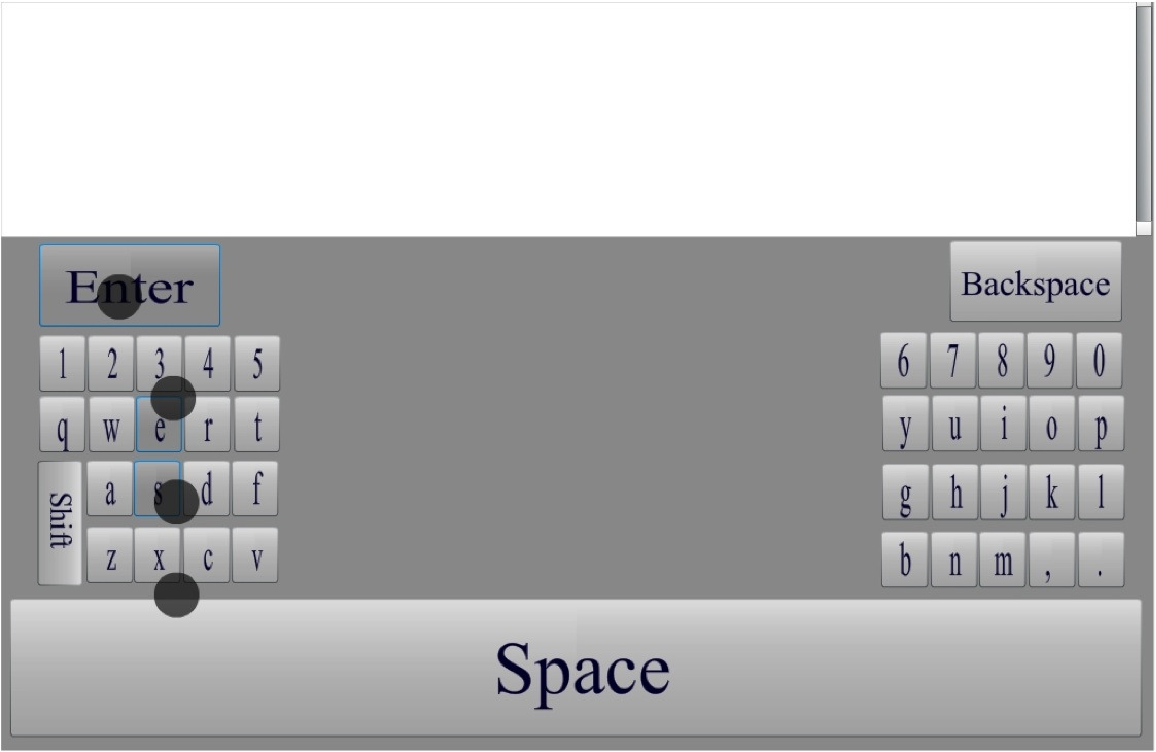
\includegraphics[scale=0.45]{Figures/backside.pdf} 
    \caption{Screenshot of backside-QWERTY with user's fingers on the
      backside screen}
\end{figure}

\subsubsection{Design evolution}

The interface went through two iterations before getting its final
shape. The first version used pressure as a method to signal
input. However, usability tests suggested that being able to control
the amount of pressure being applied is hard for users. Since the
users were already applying some pressure to drag the cursors around,
it turned out to be confusing for them.

Therefore, the second version of the interface used cursor destroy
events as a method to signal text input. In simple words, the
interface would accept a character as input if the corresponding key
had a cursor destroy event over it. However, in this case the
usability tests suggested that choosing not to give an input would
mean that the user needs to go to section of the screen that has no
keys and then choose to remove the touch/cursor. Also, the chances of
giving accidental inputs, by accidental destroy events increased
menifold. Both these factors resulted in additional overhead in terms
of time.

As a result we finally shifted to touching the front panel once the
character has been selected, as the method to signal input.

In the first version we had also modified the keyboard layout to match
the finger to key mappings on a QWERTY keyboard. However,
after the usability test, we realized that users were still doing
visual search for keys instead of using their pre-existing knowledge
of QWERTY. Therefore, a QWERTY layout in this case turned out to be
more predictable and usable.Moreover, the size of the Space, Backspace
and Enter keys was increased so that they are easy to select.

\subsection{Chording mechanism}
\subsubsection{Description}

In this mechanism the user was required to use the number of fingers
and the x-position of the fingers to signal the character that was
being entered. The screen in this case was split into 6 zones (3 on
left, 3 on right) and each zone had 3 segments. Users could switch
from one zone to the other by moving a cursor into that zone. Just
like in backside QWERTY, the users were still touching the backside
screen in order to move cursors on the front. The segments had levels
corresponding to them. The number of fingers in a particular zone
determined which level of segment the user has selected. If the user
wanted to select the first level segment in a particular zone, they
would have to move one cursor to the zone. If they wanted to select
the second level segment, they were required to move two cursors to
the corresponding zone, and so forth. Each segment on the left side of
the screen corresponded to 9 characters. The characters were organized
in an alphabetical order [Figure], so that visual search is
simplified. These 9 characters would open up on the right side if the
user selects the corresponding segment on the left. To select a
particular character that was over a segment, the user was supposed to
select the segment (as explained above) and touch anywhere on the
front screen. Therefore, each character corresponded to a unique
"chord" on each side of the screen, and therefore the mechanism was
called the chording mechanism. .  For example, in Figure 4 the user is selecting the character �l� by placing two fingers in the central region on the left hand to select the character set �jklmnopqr�, and three fingers in the right-hand region on the right hand to select �l�.  Moreover, in our implementation, the number of fingers activating a region was indicated by color changes to the activated  regions, in addition to the translucent circles representing the location of the fingers. 

The use of number of fingers, as opposed to position to select a
segment was done deliberately to restrict the movement in one
dimension. This was done in order to make sure that given enough time
the user is able to remove his eyes off the interface while entering
text. Moreover, error rate was expected to go down, because absolute
positioning was restricted to just one dimension.

Similar to backside QWERTY and QWERTY, the top quarter of the screen
was a scrollable textfield, which displayed the text that was being
entered.

\begin{figure}
    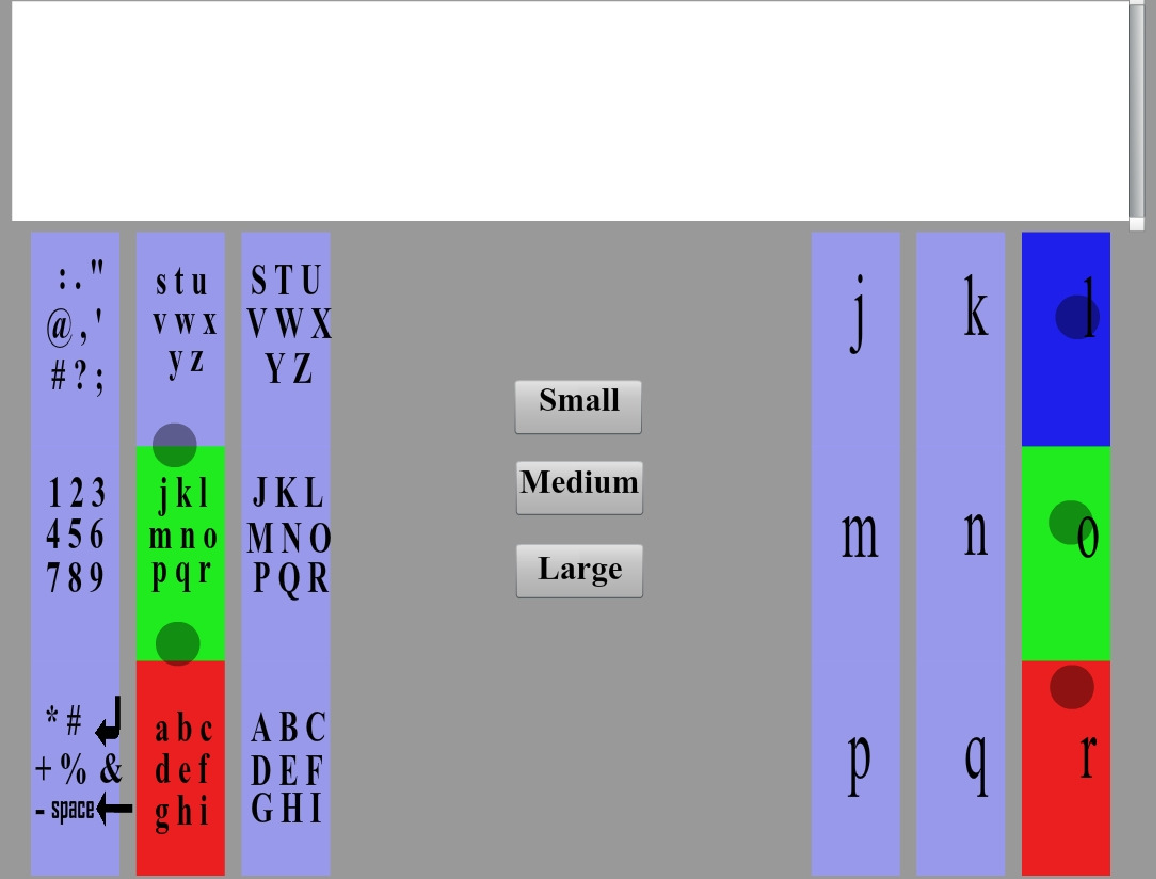
\includegraphics[scale=0.45]{Figures/chording.pdf} 
    \caption{Screenshot of chording mechanism with user's fingers on
      the backside screen trying to form a chord}
\end{figure} 
\subsubsection{Design Evolution}

As in the case of backside QWERTY, after the first round of usability
testing, it was observed that users find it hard to control the
pressure being applied by the fingers. Therefore, in the final version
of the mechanism the users could touch the front screen to signal text
input for the character selected by the chords.

Usability testing suggested that the finger sizes and areas in which
users can move comfortably vary a lot. Therefore, in the final version
the users were allowed to select from large/medium/small setting
[Figure], that determined the width of the zones. Users, who had
smaller reach, could use these settings to optimize the area of
movement.
